\chapter{Conclusion}
\label{chap:concl}

\section{Conclusion}

The aim of this study was to design and test a machine learning-based model to predict the
post-harvest loss risk among smallholder agribusinesses in developing nations, specifically Nigeria,
based on LSMS-ISA data~\cite{ghspanel2024nigeria}. This study focused on answering three major
research questions: understanding the principal determinants of post-harvest losses, determining the
predictive performance of simple machine learning models, and determining how those predictions can
be used to inform viable agribusiness management decisions.

The results show that post-harvest losses are still a major menace, with a large percentage of
smallholder farmers being affected. The analysis showed that storage-related variables, especially
storage method and length of storage, are the most crucial factors of loss risk. Type of crop and
geographic location are also important factors which introduce differences attributable to
perishability and infrastructure facilities. These findings affirm the hypothesis that post-harvest
losses are determined by a set of operational, environmental, and socio-economic factors.

Regarding predictive modelling, the researchers discovered that simple machine learning models are
capable of attaining high levels of accuracy with structured tabular data. The best of the models
analysed was the Random Forest, which showed a greater capacity to compute non-linear, complex
relationships between variables. The Decision Tree also demonstrated high performance and presented
useful interpretability, while Logistic Regression offered a strong baseline. These lessons show
that resource-consuming and complex tools are not always necessary for effective predictive
performance.

Significantly, the research revealed that machine learning predictions may be converted into
agribusiness action insights. The high-risk situations can be determined, helping farmers to make
the right choices about whether to store, handle, and sell products at the right time. This
supports the development of low-cost decision support systems in smallholder scenarios, helping to
develop efficiency and minimize losses. In general, the study fulfills its purpose, as it offers a
feasible data-based model to forecast the risk of post-harvest losses. It adds to the academic and
practical knowledge base, pointing to the possibilities of accessible machine learning solutions
in solving critical agricultural problems.


\section{Recommendations}

This research presents a number of recommendations to farmers, policymakers, and future research
bases, based on the findings of this study.

\subsection{Recommendations for Smallholder Farmers}

Smallholder farmers should first improve storage practices, since the method of storage and storage
time were recognized as the most effective predictors of post-harvest losses. Even at the simplest
level, adoption of better storage technologies can make a great difference in the reduction of
spoilage. The farmers can also reduce storage time where possible, and should handle produce
properly on harvesting and transportation as a way of minimising mechanical damage. Additionally,
crop-specific measures must be embraced, especially for highly perishable crops that require
careful handling.

\subsection{Recommendations for Policymakers and Institutions}

To manage structural aspects of post-harvest losses, policymakers ought to invest in rural
infrastructure, especially storage and transport facilities. They should use training programmes to
inform the farmers on best practices in post-harvest management. Additionally, it is necessary to
facilitate the design and implementation of straightforward digital decision support systems that
can offer real-time information to farmers using data. Agencies and other organizations in the
agricultural sector should also enable access to agricultural data and encourage data-driven
solutions. Enhancement of partnerships between the research and agriculture communities can bolster
the incorporation of new agricultural solutions.

\subsection{Recommendations for Future Research}

Further investigation is recommended to enhance the scope of this study. Diversification of data
is necessary since this study focuses on one country; future work should incorporate more extensive
and intersecting databases covering multiple regions. Predictive accuracy could be further improved
through the incorporation of environmental variables like temperature and rainfall. Moreover, the
application of more sophisticated machine learning methods, including deep learning, could be
explored while keeping interpretability and computational cost in mind. It is also necessary to
build and test real-time decision support systems using the models presented in this research paper.
This would help close the gap between theoretical and practical research, ensuring that predictive
knowledge is converted into actionable outcomes.


\section{Final Reflection}

This paper has explained the mechanism by which agricultural knowledge and machine learning could
help to solve one of the most pressing problems in the developing countries. The research
demonstrates that much can be achieved with a strategic focus on simplicity, accessibility, and
usability of solutions, and that effective technological tools do not necessarily require complex
infrastructure. To sum up, the minimization of post-harvest losses is a challenge of both technical
and social character, and it is a pathway toward better food security, the improved livelihoods of
farmers, and the sustainable development of agriculture.


% =============================================================
% Appendix
% =============================================================
\appendix
\chapter{Supplementary Figures}
\label{app:figures}

This appendix contains supplementary output figures from the machine learning analysis, including
additional model diagnostics, exploratory data analysis charts, and visualizations generated during
the computational experiments.

\begin{figure}[htbp]
    \centering
    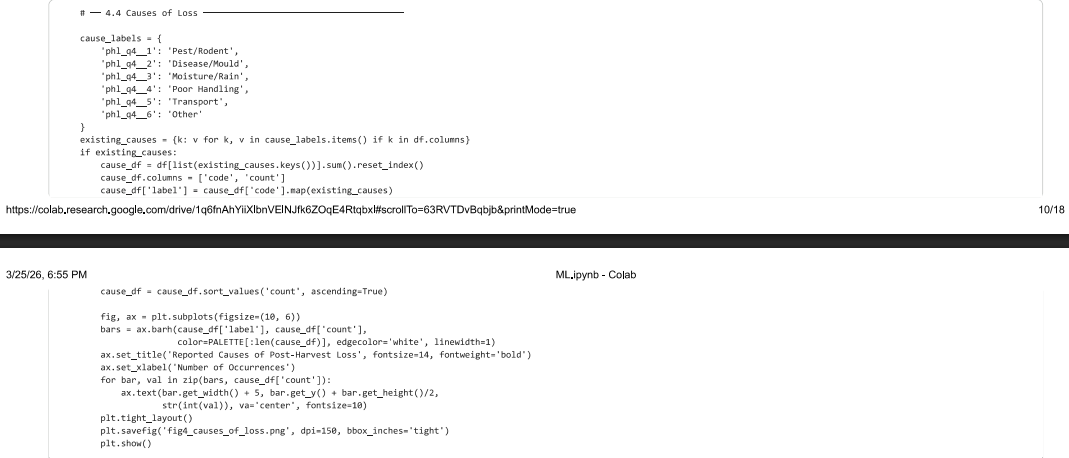
\includegraphics[width=\textwidth]{attachments/figures/image10}
    \caption{Supplementary Figure 1}
    \label{fig:app1}
\end{figure}

\begin{figure}[htbp]
    \centering
    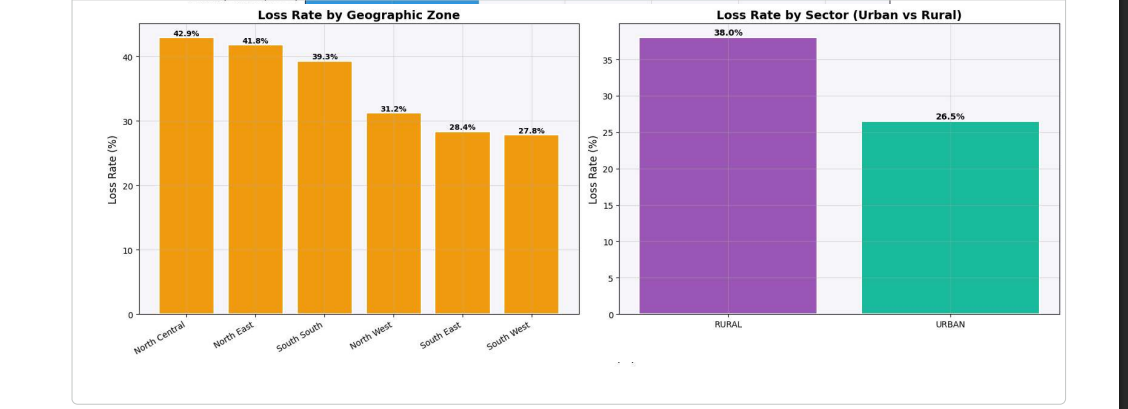
\includegraphics[width=\textwidth]{attachments/figures/image11}
    \caption{Supplementary Figure 2}
    \label{fig:app2}
\end{figure}

\begin{figure}[htbp]
    \centering
    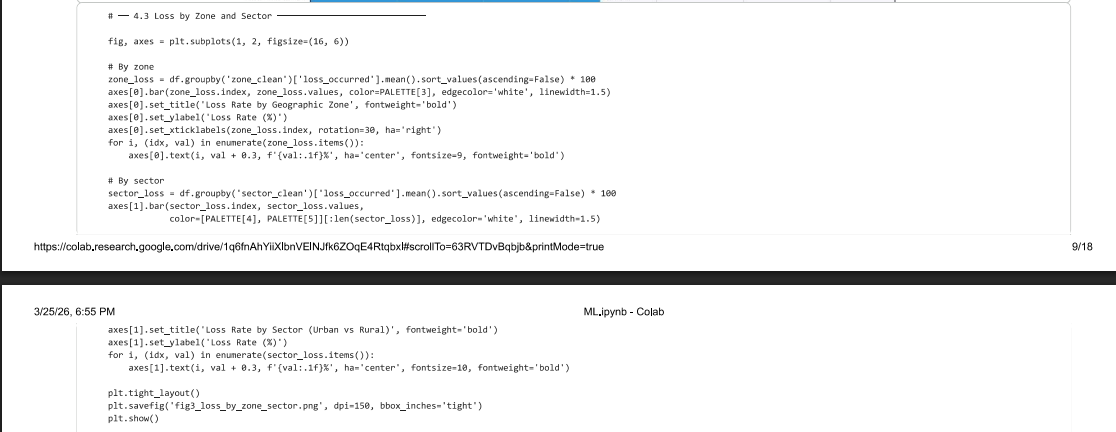
\includegraphics[width=\textwidth]{attachments/figures/image12}
    \caption{Supplementary Figure 3}
    \label{fig:app3}
\end{figure}

\begin{figure}[htbp]
    \centering
    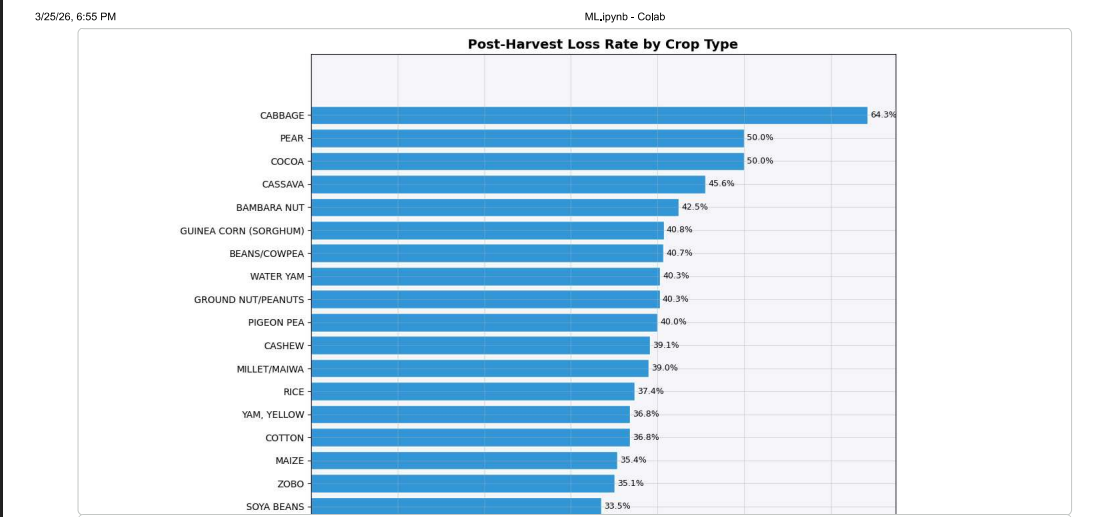
\includegraphics[width=\textwidth]{attachments/figures/image13}
    \caption{Supplementary Figure 4}
    \label{fig:app4}
\end{figure}

\begin{figure}[htbp]
    \centering
    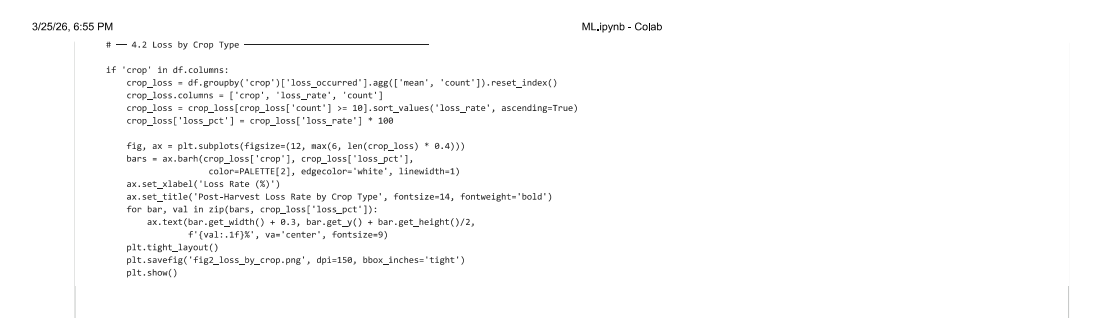
\includegraphics[width=\textwidth]{attachments/figures/image14}
    \caption{Supplementary Figure 5}
    \label{fig:app5}
\end{figure}

\begin{figure}[htbp]
    \centering
    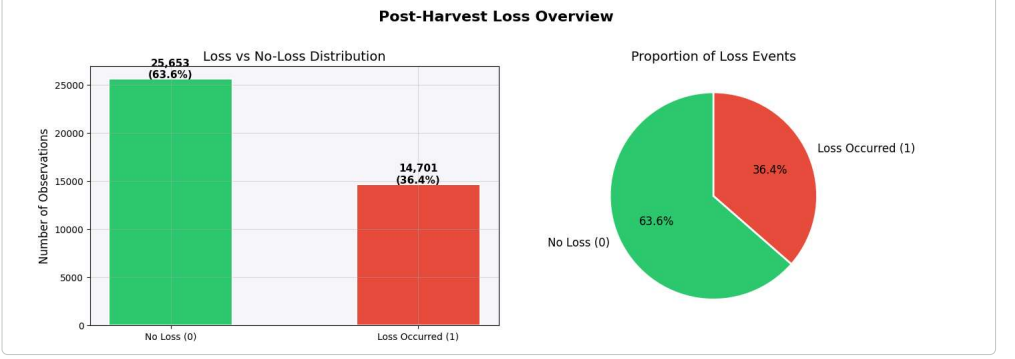
\includegraphics[width=\textwidth]{attachments/figures/image15}
    \caption{Supplementary Figure 6}
    \label{fig:app6}
\end{figure}

\begin{figure}[htbp]
    \centering
    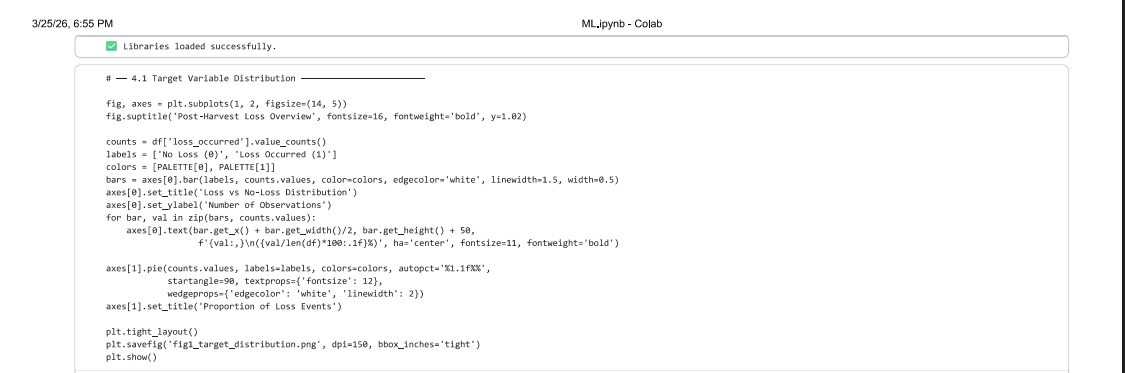
\includegraphics[width=\textwidth]{attachments/figures/image16}
    \caption{Supplementary Figure 7}
    \label{fig:app7}
\end{figure}

\begin{figure}[htbp]
    \centering
    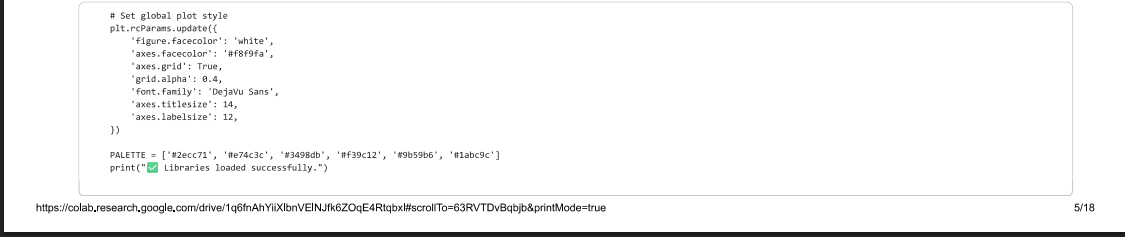
\includegraphics[width=\textwidth]{attachments/figures/image17}
    \caption{Supplementary Figure 8}
    \label{fig:app8}
\end{figure}

\begin{figure}[htbp]
    \centering
    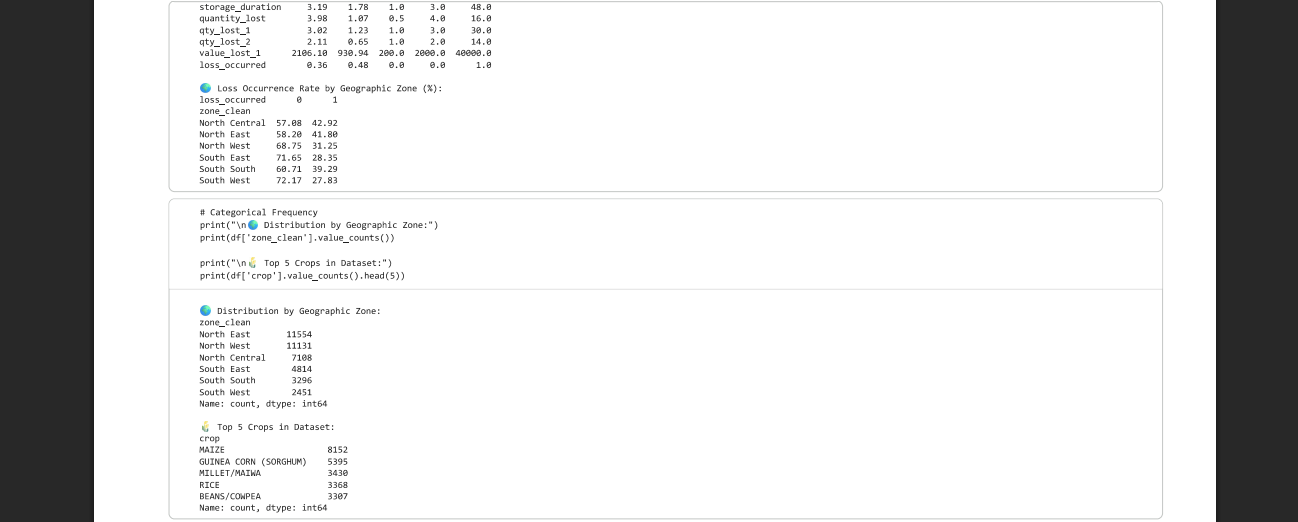
\includegraphics[width=\textwidth]{attachments/figures/image18}
    \caption{Supplementary Figure 9}
    \label{fig:app9}
\end{figure}

\begin{figure}[htbp]
    \centering
    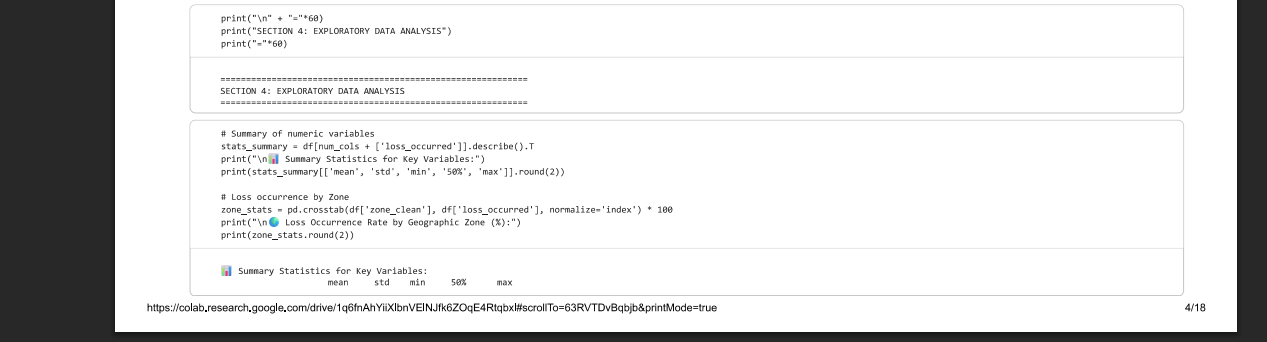
\includegraphics[width=\textwidth]{attachments/figures/image19}
    \caption{Supplementary Figure 10}
    \label{fig:app10}
\end{figure}

\begin{figure}[htbp]
    \centering
    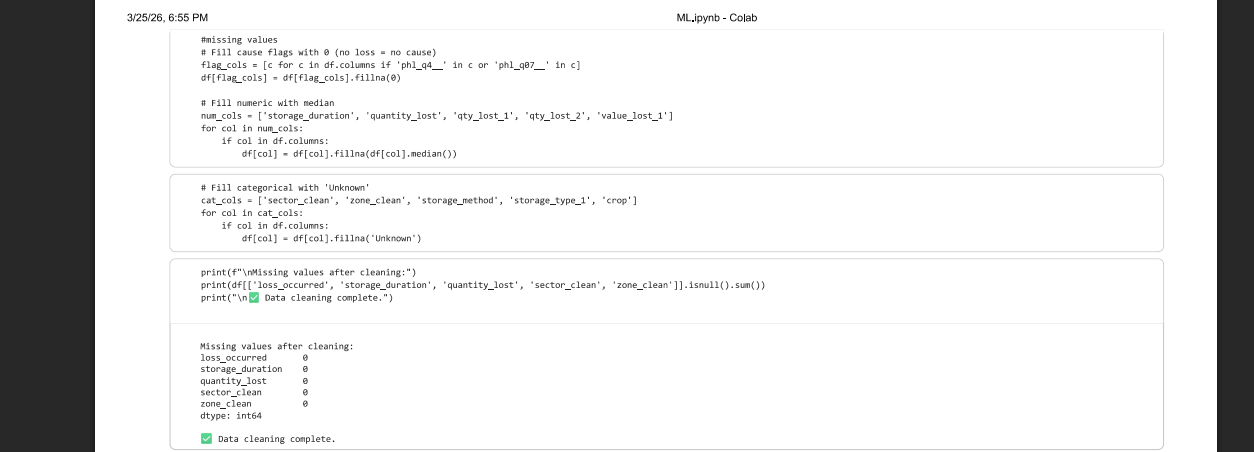
\includegraphics[width=\textwidth]{attachments/figures/image20}
    \caption{Supplementary Figure 11}
    \label{fig:app11}
\end{figure}

\begin{figure}[htbp]
    \centering
    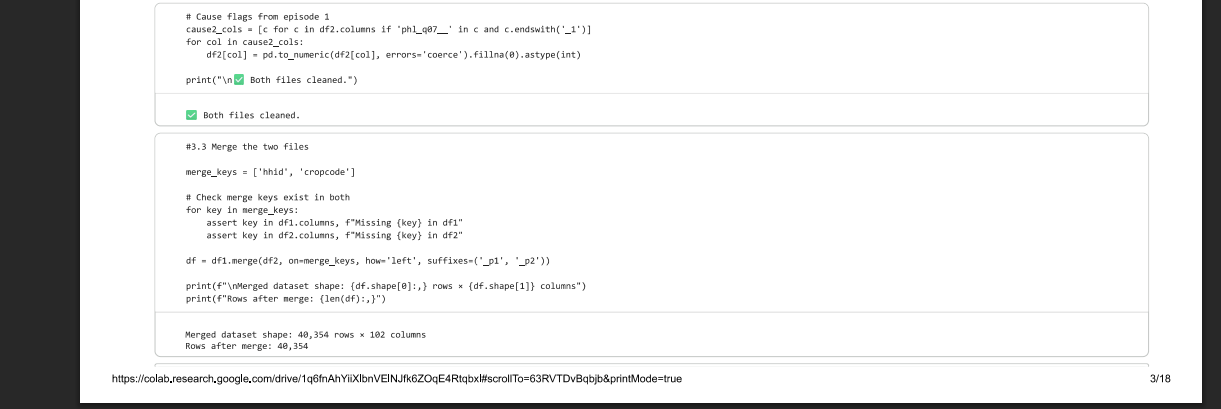
\includegraphics[width=\textwidth]{attachments/figures/image21}
    \caption{Supplementary Figure 12}
    \label{fig:app12}
\end{figure}

\begin{figure}[htbp]
    \centering
    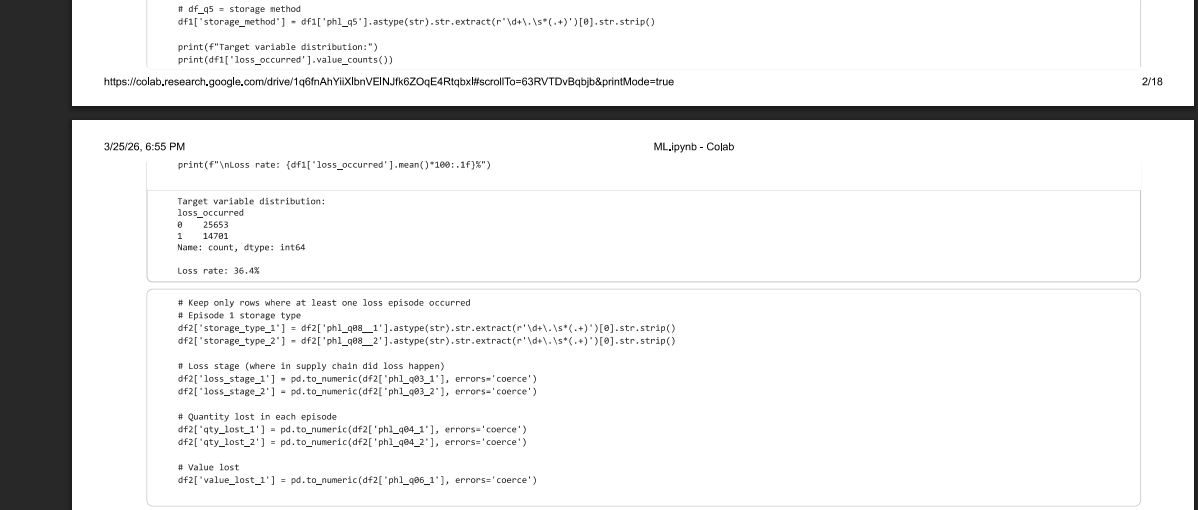
\includegraphics[width=\textwidth]{attachments/figures/image22}
    \caption{Supplementary Figure 13}
    \label{fig:app13}
\end{figure}

\begin{figure}[htbp]
    \centering
    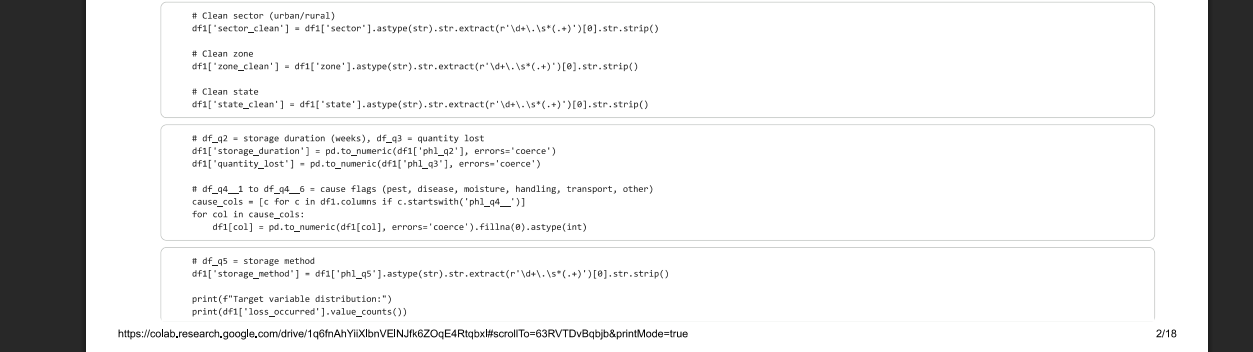
\includegraphics[width=\textwidth]{attachments/figures/image23}
    \caption{Supplementary Figure 14}
    \label{fig:app14}
\end{figure}

\begin{figure}[htbp]
    \centering
    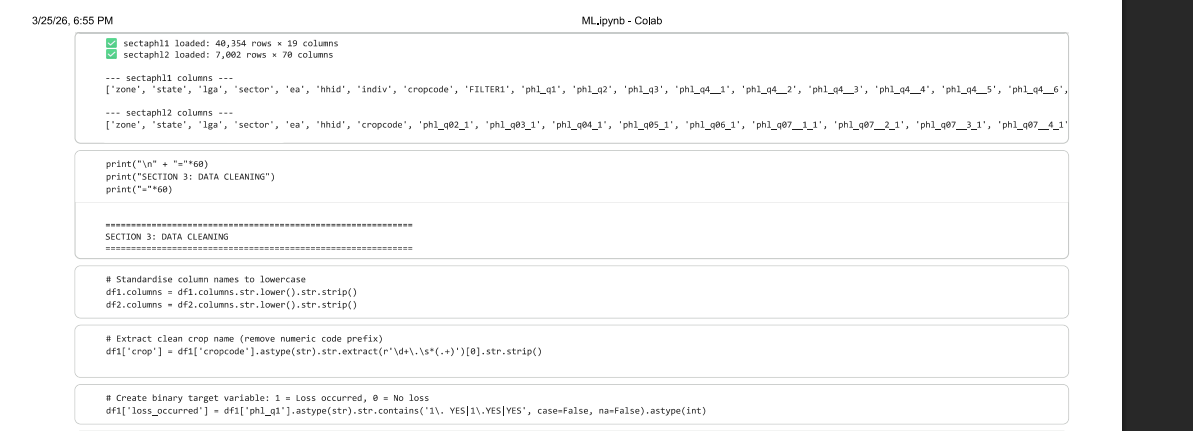
\includegraphics[width=\textwidth]{attachments/figures/image24}
    \caption{Supplementary Figure 15}
    \label{fig:app15}
\end{figure}

\begin{figure}[htbp]
    \centering
    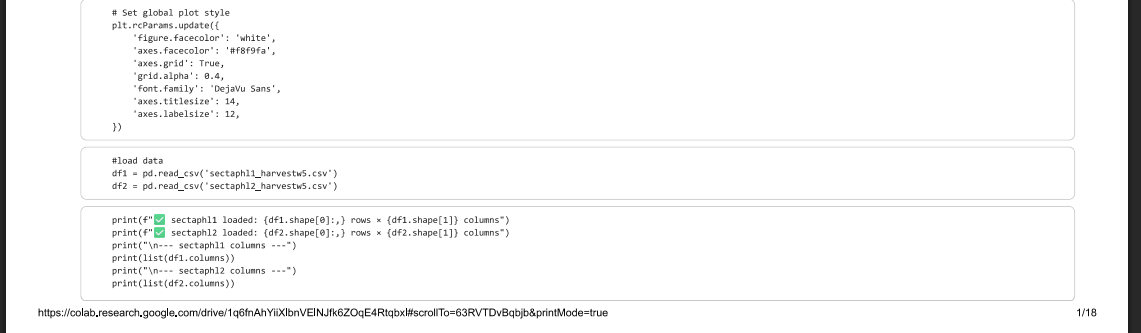
\includegraphics[width=\textwidth]{attachments/figures/image25}
    \caption{Supplementary Figure 16}
    \label{fig:app16}
\end{figure}

\begin{figure}[htbp]
    \centering
    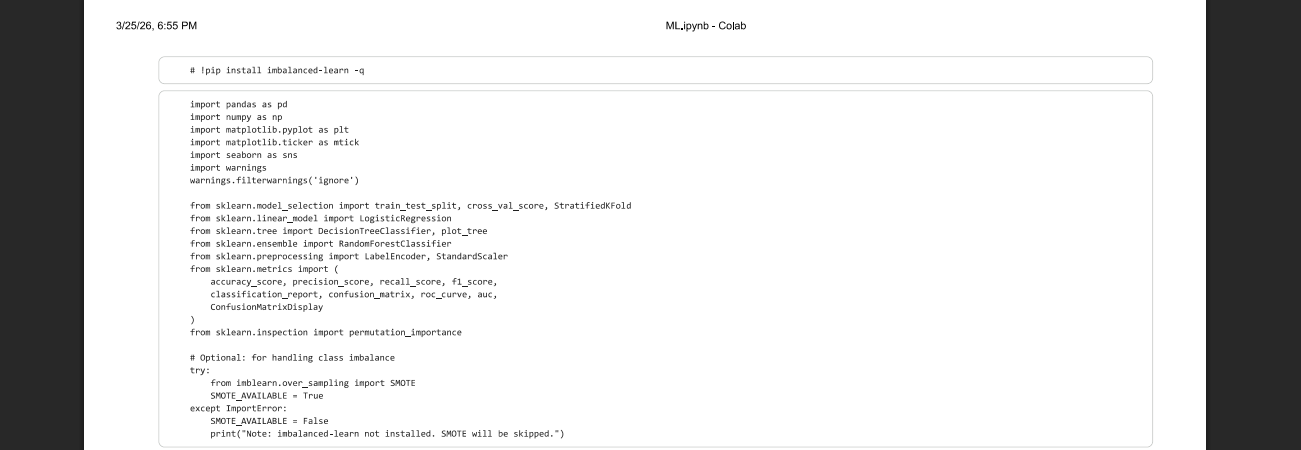
\includegraphics[width=\textwidth]{attachments/figures/image26}
    \caption{Supplementary Figure 17}
    \label{fig:app17}
\end{figure}

\begin{figure}[htbp]
    \centering
    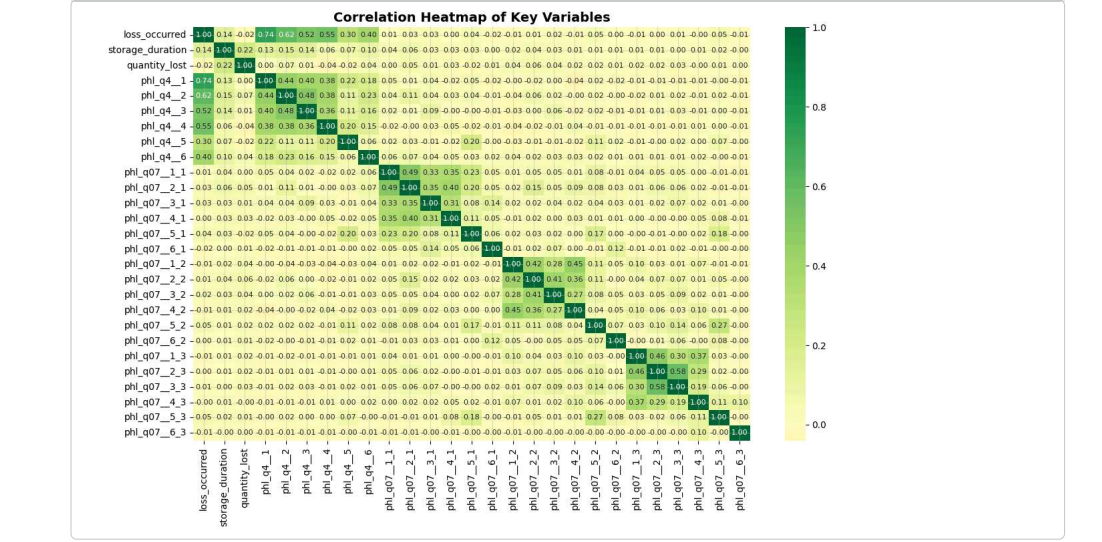
\includegraphics[width=\textwidth]{attachments/figures/image27}
    \caption{Supplementary Figure 18}
    \label{fig:app18}
\end{figure}

\begin{figure}[htbp]
    \centering
    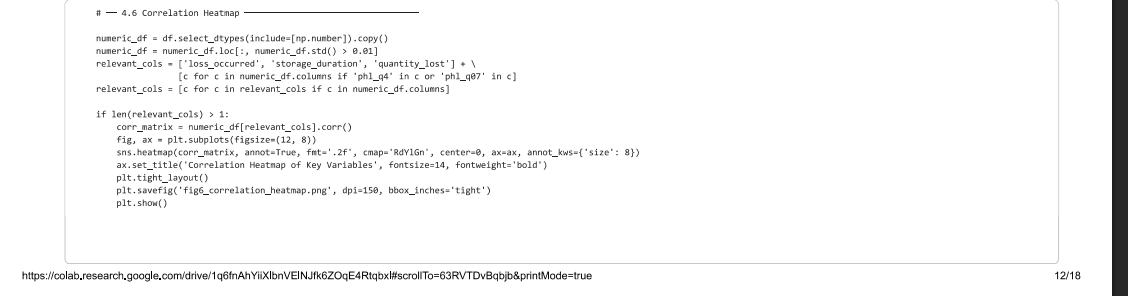
\includegraphics[width=\textwidth]{attachments/figures/image28}
    \caption{Supplementary Figure 19}
    \label{fig:app19}
\end{figure}

\begin{figure}[htbp]
    \centering
    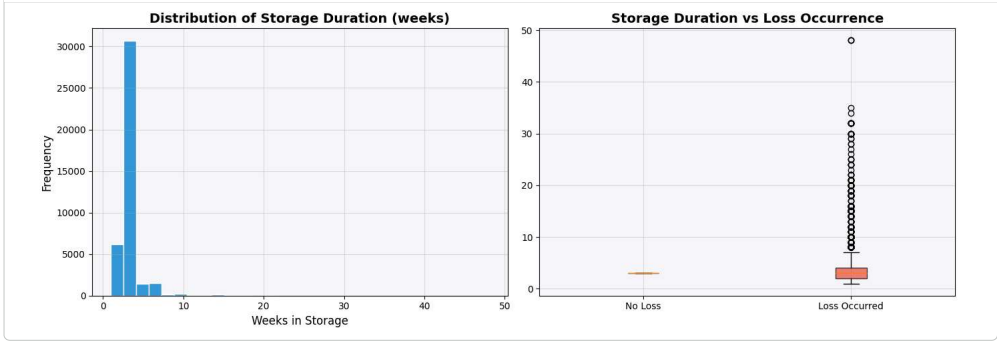
\includegraphics[width=\textwidth]{attachments/figures/image29}
    \caption{Supplementary Figure 20}
    \label{fig:app20}
\end{figure}

\begin{figure}[htbp]
    \centering
    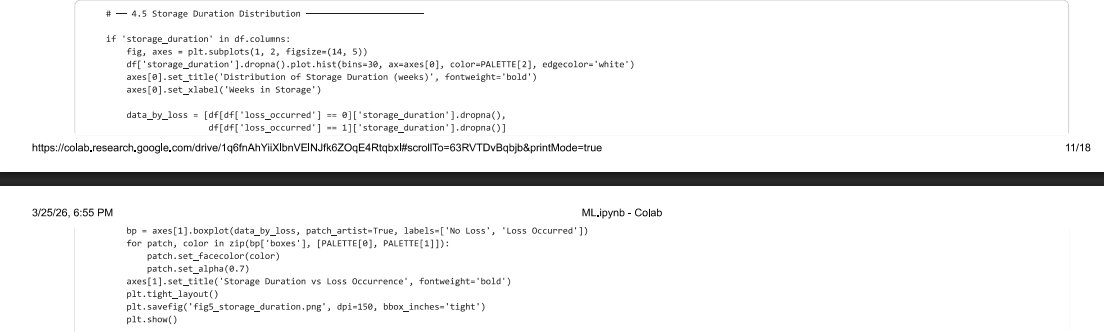
\includegraphics[width=\textwidth]{attachments/figures/image30}
    \caption{Supplementary Figure 21}
    \label{fig:app21}
\end{figure}

\begin{figure}[htbp]
    \centering
    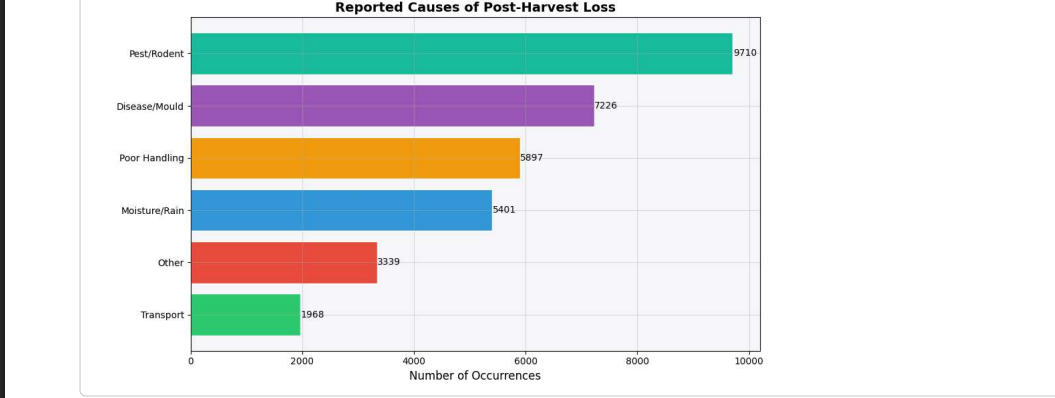
\includegraphics[width=\textwidth]{attachments/figures/image31}
    \caption{Supplementary Figure 22}
    \label{fig:app22}
\end{figure}

\begin{figure}[htbp]
    \centering
    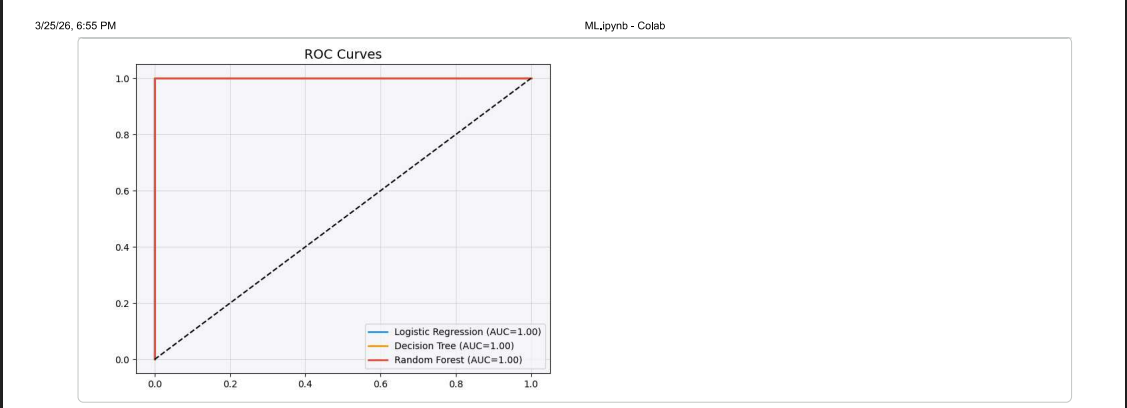
\includegraphics[width=\textwidth]{attachments/figures/image32}
    \caption{Supplementary Figure 23}
    \label{fig:app23}
\end{figure}

\begin{figure}[htbp]
    \centering
    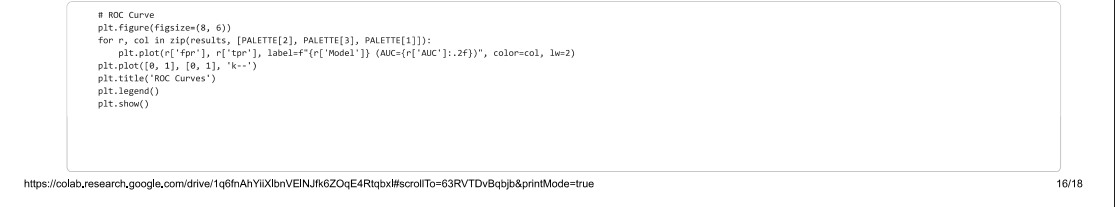
\includegraphics[width=\textwidth]{attachments/figures/image33}
    \caption{Supplementary Figure 24}
    \label{fig:app24}
\end{figure}

\begin{figure}[htbp]
    \centering
    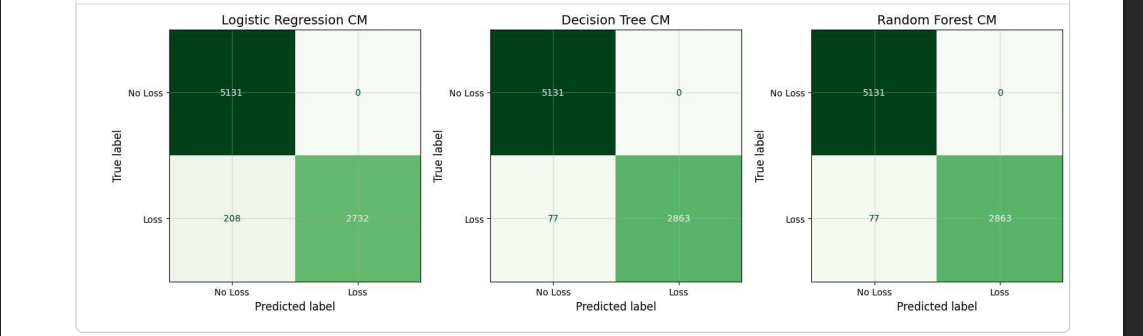
\includegraphics[width=\textwidth]{attachments/figures/image34}
    \caption{Supplementary Figure 25}
    \label{fig:app25}
\end{figure}

\begin{figure}[htbp]
    \centering
    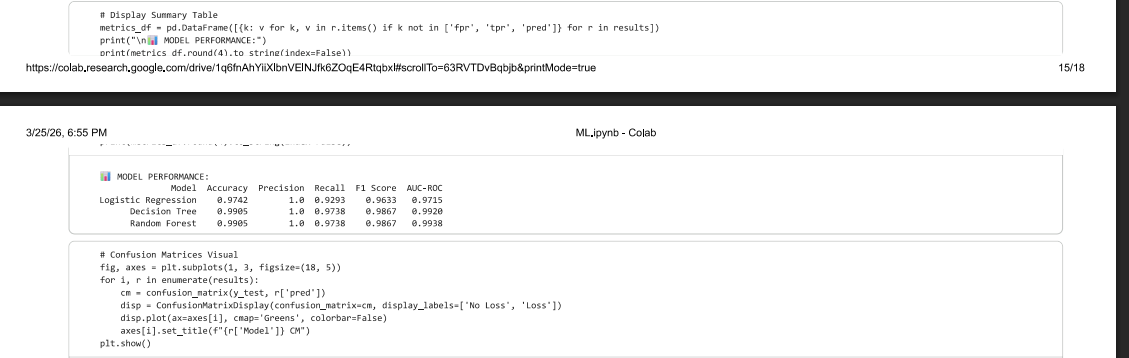
\includegraphics[width=\textwidth]{attachments/figures/image35}
    \caption{Supplementary Figure 26}
    \label{fig:app26}
\end{figure}

\begin{figure}[htbp]
    \centering
    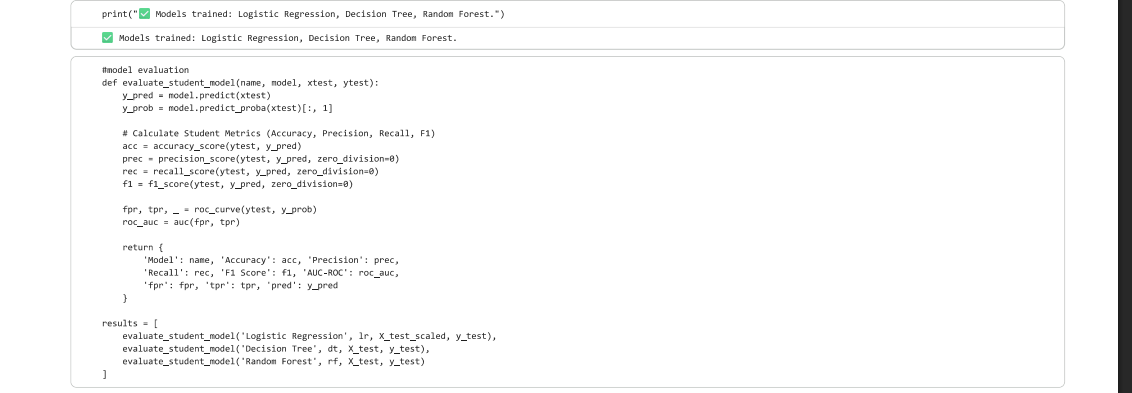
\includegraphics[width=\textwidth]{attachments/figures/image36}
    \caption{Supplementary Figure 27}
    \label{fig:app27}
\end{figure}

\begin{figure}[htbp]
    \centering
    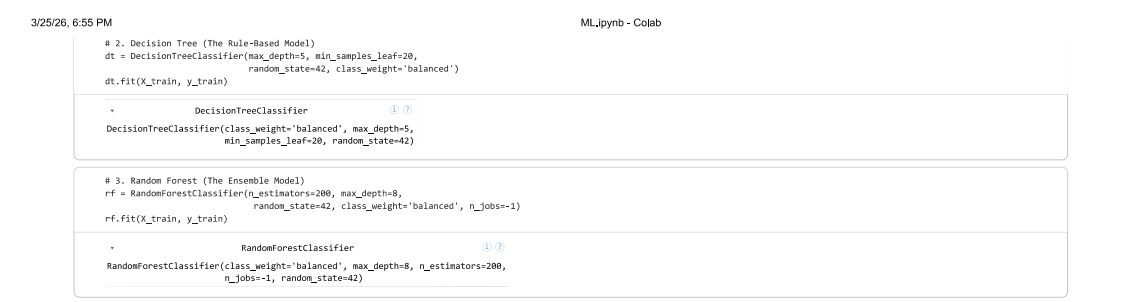
\includegraphics[width=\textwidth]{attachments/figures/image37}
    \caption{Supplementary Figure 28}
    \label{fig:app28}
\end{figure}

\begin{figure}[htbp]
    \centering
    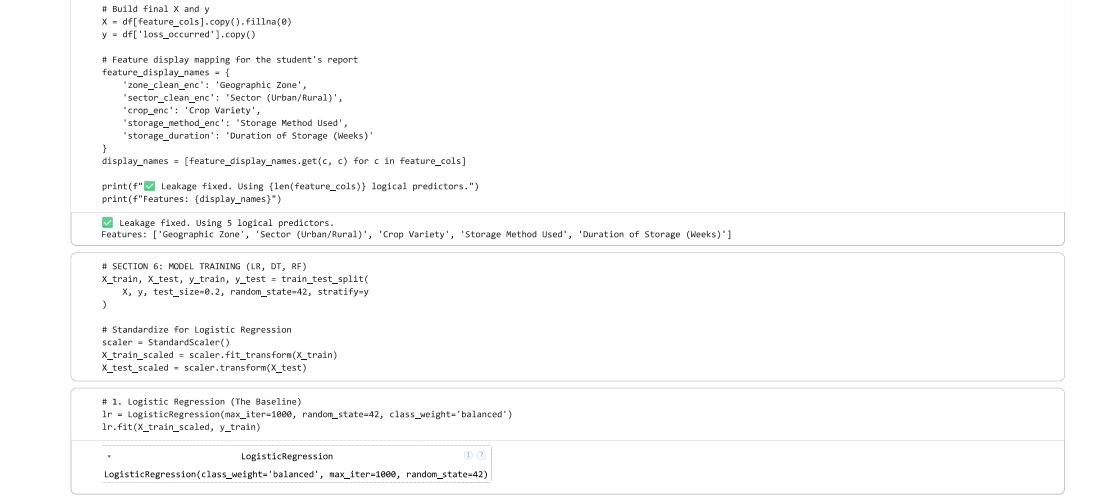
\includegraphics[width=\textwidth]{attachments/figures/image38}
    \caption{Supplementary Figure 29}
    \label{fig:app29}
\end{figure}

\begin{figure}[htbp]
    \centering
    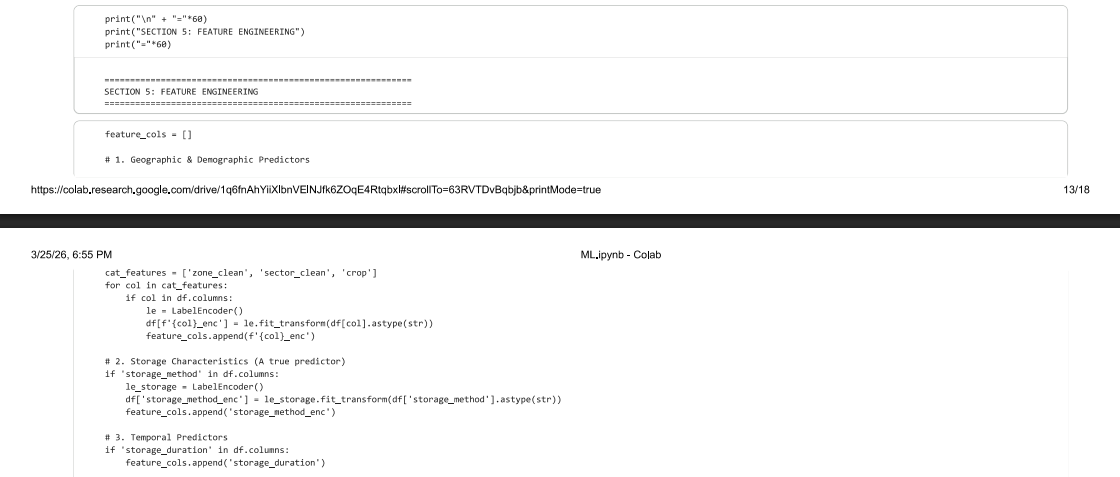
\includegraphics[width=\textwidth]{attachments/figures/image39}
    \caption{Supplementary Figure 30}
    \label{fig:app30}
\end{figure}

\begin{figure}[htbp]
    \centering
    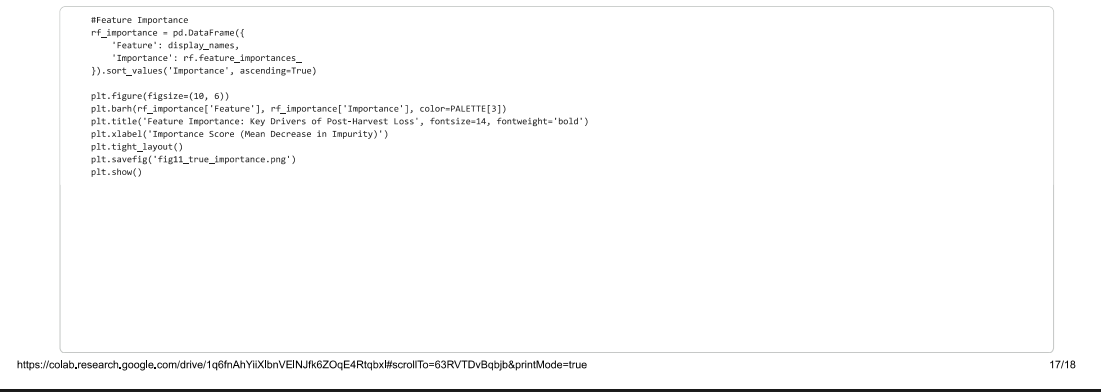
\includegraphics[width=\textwidth]{attachments/figures/image40}
    \caption{Supplementary Figure 31}
    \label{fig:app31}
\end{figure}
